\section{Discussion}\label{discuss}
%VI.	Discussion
%	a.	\pacora in the Cloud
%	b.	Challenges
%		i.	Outliers/Performance Non-Monotonicity
%			1.	Possible Solutions
%				a.	Heuristics + Feedback
%				b.	Stochastic Models
%		ii.	Variability - can't just average
%			1.	Phases
%			2.	Input Dependent
%			3.	Other � such as network connection
%			4.	Shared Resources
%			5.	Possible Solutions
%				a.	Heuristics + Feedback
%				b.	Stochastic Models
%				c.	Changing Models

\subsection*{\pacora for Warehouse-Scale Computing}
Discuss major differences, particularly storage

\subsection*{Challenges}
\subsubsection*{Outliers and Performance Non-Monotonicity}
Figure~\ref{accuracy_quality} shows the effect of model accuracy on the quality of the resource allocation decisions made.
\begin{figure*}[!t]
	\begin{center}	
%		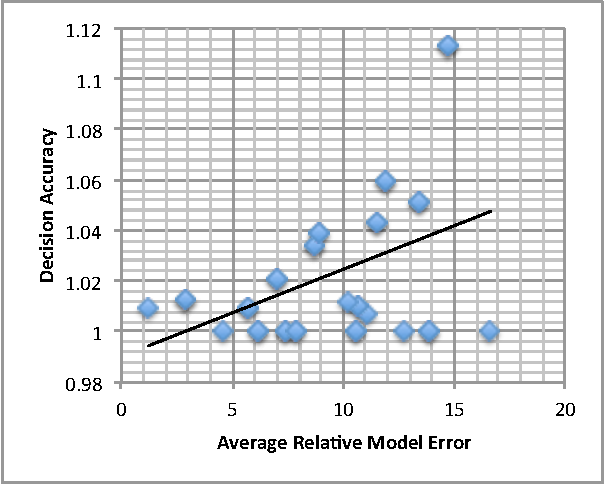
\includegraphics[width=.45\textwidth]{cluster_decision_accuracy.pdf}
%		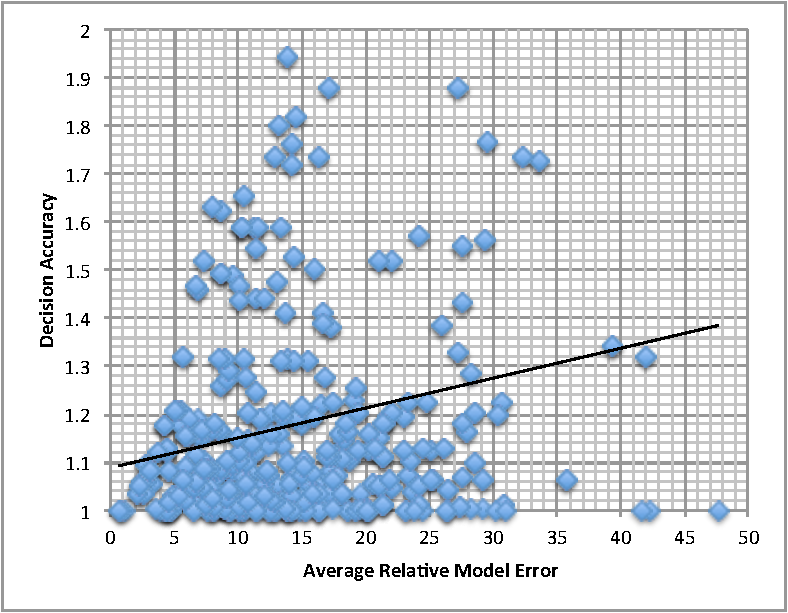
\includegraphics[width=.45\textwidth]{parsec_decision_accuracy.pdf}
		\caption{Effect of Model Accuracy on Decision Quality}
		\label{accuracy_quality}
	\end{center}
\end{figure*}

Discuss Heuristics + Feedback
\subsubsection*{Variability}
Discuss phases, input dependence, other variability (such as network connection), shared resources

Possible solutions include Heuristics + Feedback, Stochastic Models, Changing Models

%Program phase detection has targeted hardware or software reconfiguration. The overview~\cite{dhodapkar-micro03} evaluates three measurement-based predictors, and while performance variation is not one of the three, the authors note that small performance variation is an indicator of correct phase identification.  A similar conclusion is reached in~\cite{sherwood-sigarch03}.

% don't forget cpu frequency




